Crowdsourcing video annotation approaches are used in various applications and are used to gather information of various types, such as temporal synchronization\cite{wu2014crowdsourced,wfa2016}, events\cite{Kim:2014:JSL:2679600.2680027,sulser2014crowd}, scene objects\cite{vidwiki2014,pinto2013tag4vd}, emotions\cite{sanchez2015mood,biel2013youtube}, actions\cite{riek2011guess,desell2015effectiveness}, quality\cite{freiburg2011crowdsourcing,han2014quality}, geo-tagging\cite{chen2015crowd,gottlieb2012pushing}, social relevance\cite{santos2014towards,huron2013polemictweet,bertini2013socially} and captions\cite{deshpande2014crowdsourcing,kacorri2014introducing}. 

However, some of these works are based on complex annotation tools, demanding hard, tedious or time-consuming tasks, or requiring trained and skilled workers. Some relevant examples that should be regarded include works such as \cite{vidwiki2014,Vondrick:2013:ESU:2436010.2436013,park2014toward,biel2013youtube,desell2015effectiveness,gottlieb2012pushing,huron2013polemictweet}.

VidWiki\cite{vidwiki2014} is a complex system to improve video lesson by video annotation, which provides a complex annotation tool(Figure~\ref{related_1_a}) that allows the worker to edit video scenes by adding various types of annotations, including LaTex equations. Another interesting paper to note was written in 2012 by C.Vandrick\cite{Vondrick:2013:ESU:2436010.2436013}, in which time-consuming complex tasks were deployed in the Amazon Mechanical Turk\cite{gottlieb2012pushing} demanding specialized work to perform them. 

While these works often produce interesting results, to adopt complex annotation tools, as well as hard and time-consuming tasks, restrict potential workers and owners capable of developing complex tools and hiring skilled workers.

\begin{figure}[h]
	\centerline{\includegraphics[scale=0.21] {figure/related_1_a}}
	\caption{VidWiki annotation tool\cite{vidwiki2014}}
	\label{related_1_a}
\end{figure} 

There are also papers on crowdsourcing video annotation that report the use of simple tools and microtasks that can be done quickly by unskilled workers. These works include \cite{Chen:2017:RIM:3025453.3025969,Kim:2014:JSL:2679600.2680027,riek2011guess,gadgil2014web,wfa2016,wu2014crowdsourced,pinto2013tag4vd,sulser2014crowd}.

The work published by N.Gagil in 2014\cite{gadgil2014web} uses a very simple annotation tool(Figure~\ref{related_d}) that allows the workers to perform an easy microtask, which consists of annotate videos with surveillance problems if any of them are found.

\begin{figure}[h]
	\centerline{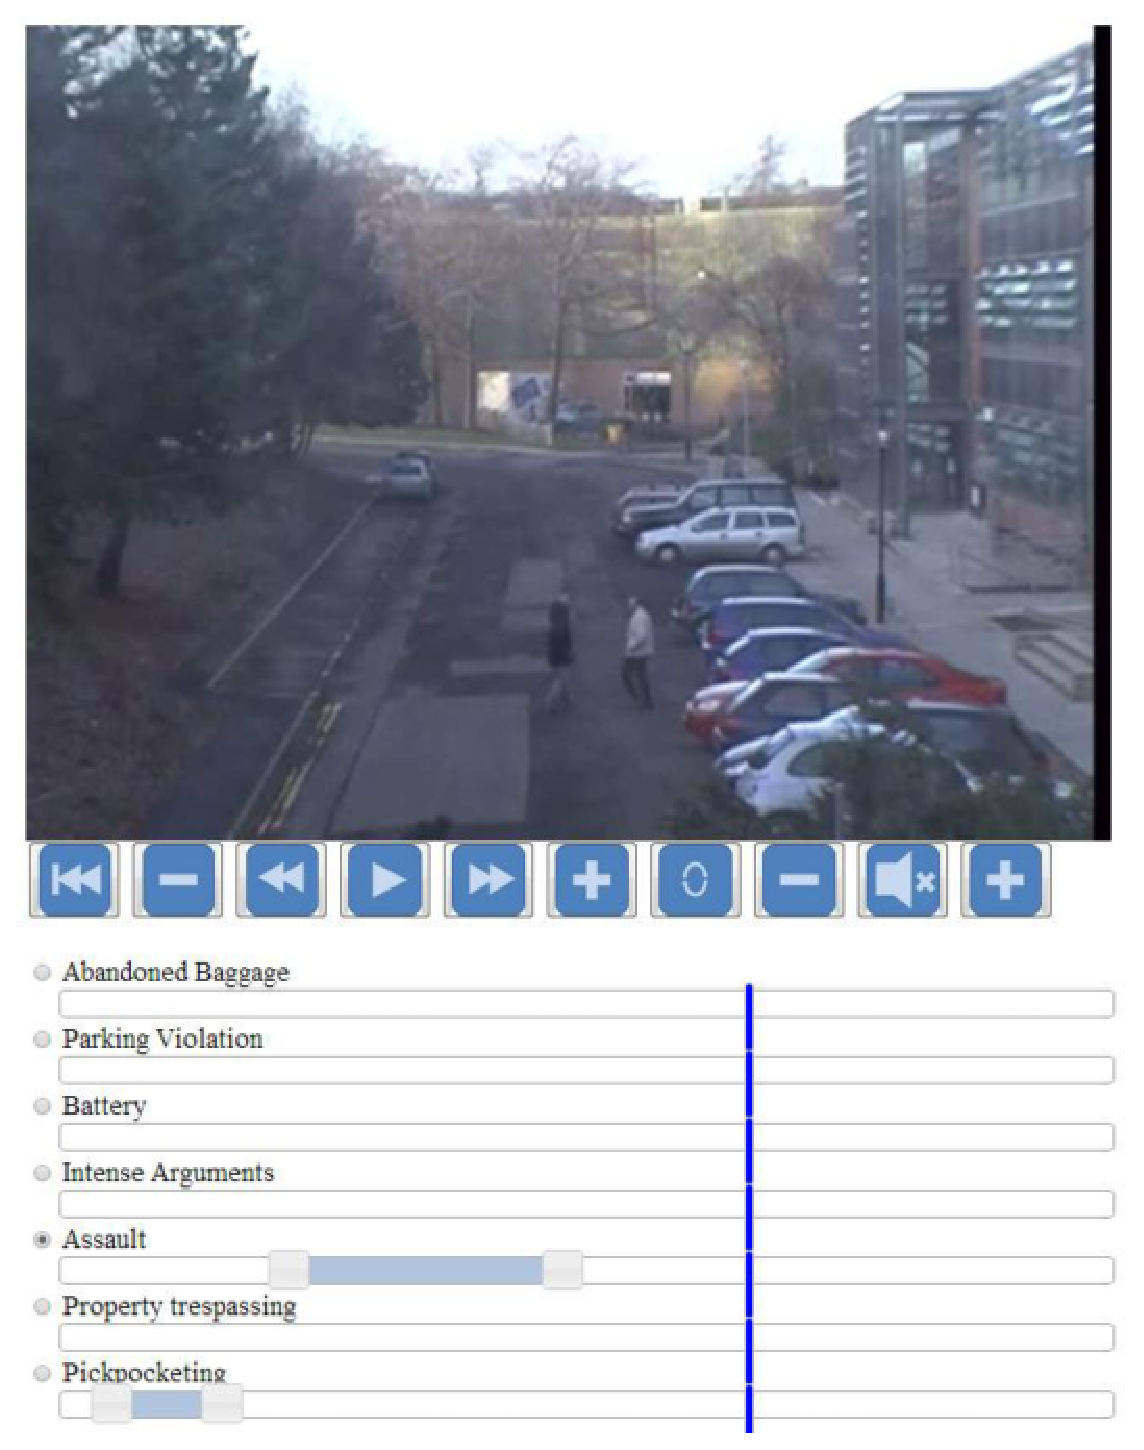
\includegraphics[scale=0.3] {figure/related_d}}
	\caption{Simple surveillance annotation tool\cite{gadgil2014web}}
	\label{related_d}
\end{figure} 

ReTool\cite{Chen:2017:RIM:3025453.3025969} is a work that must be mentioned, because it presents a web-based tool for owners to create and publish annotation microtasks and workflows to execute them.

ToolScape\cite{Kim:2014:JSL:2679600.2680027} is a work that deserves prominence, as it is strongly related to the approach presented in this paper. ToolScape integrates simple annotation tools in which workers can perform a sequence of three microtasks, that was used to extract the step-by-step structure of the instruction videos, one of these tools is shown on Figure~\ref{related_2_a}. Moreover, is presented a design pattern to define the workflow for these tasks.

\begin{figure}[h]
	\centerline{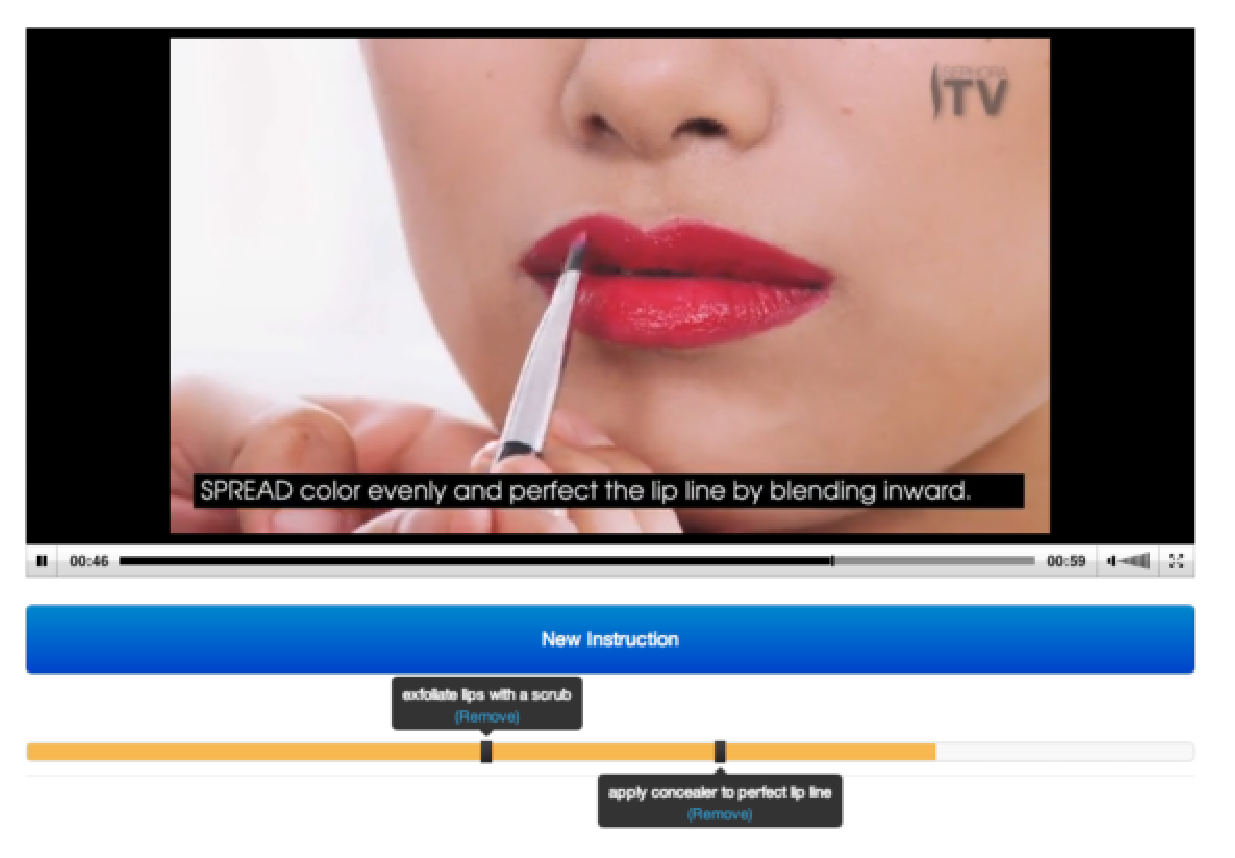
\includegraphics[scale=0.23] {figure/related_2_a}}
	\caption{ToolScape annotation tool\cite{Kim:2014:JSL:2679600.2680027}}
	\label{related_2_a}
\end{figure} 

This brief discussion about some related works aims mainly to highlight the characteristics of the microtasks, as well as the simple annotation tools used to execute them.